83. $\cfrac{((x^2-4)^2+y^2+2y+1)(y^2-4xy+3x^2)}{xy-2y+2x-4}=0\Leftrightarrow
\begin{cases}
((x^2-4)^2+y^2+2y+1)(y^2-4xy+3x^2)=0,\\
xy-2y+2x-4\neq0.
\end{cases}$\\$\Leftrightarrow
\begin{cases}
\left[\begin{array}{l}
(x^2-4)^2+(y+1)^2=0,\\
y(y-x)+3x(x-y)=0,
\end{array}\right.\\
y(x-2)+2(x-2)\neq0.
\end{cases}\Leftrightarrow
\begin{cases}
\left[\begin{array}{l}
\begin{cases}
x^2-4=0,\\
y+1=0.
\end{cases}\\
(y-x)(y-3x)=0,
\end{array}\right.\\
(x-2)(y+2)\neq0.
\end{cases}\Leftrightarrow
\begin{cases}
\left[\begin{array}{l}
\begin{cases}
x=2,\\
y=-1.
\end{cases}\\
\begin{cases}
x=-2,\\
y=-1.
\end{cases}\\
y=x,\\
y=3x,
\end{array}\right.\\
x\neq2,\\
y\neq-2.
\end{cases}$
\begin{figure}[ht!]
\center{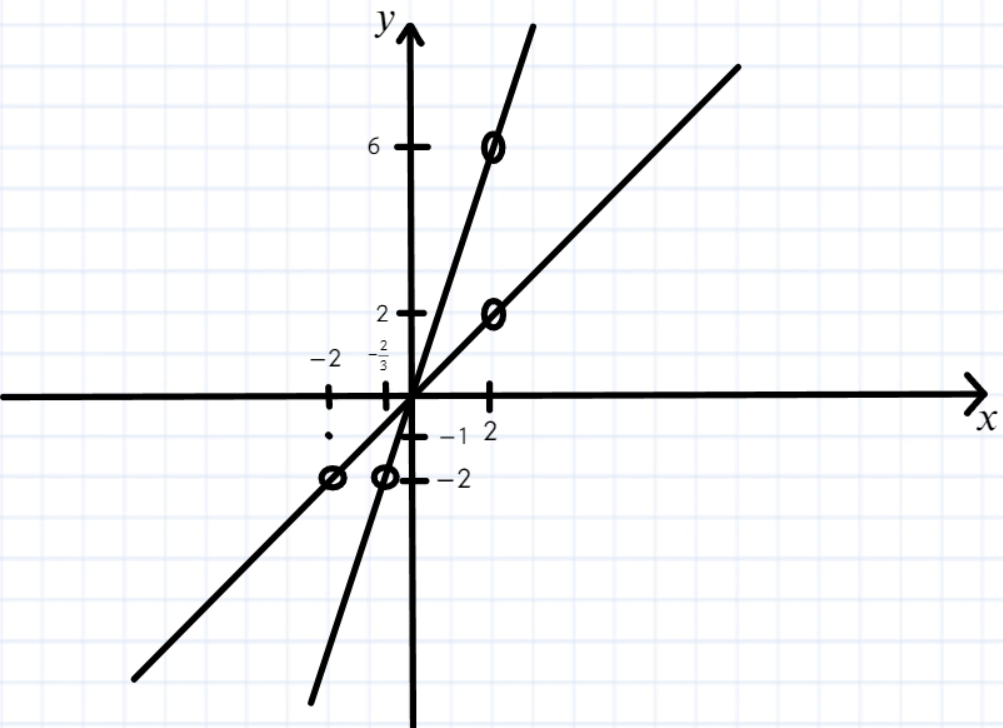
\includegraphics[scale=0.35]{gr7-83.png}}
\end{figure}\\
